% Level

Level errors (as defined in \secref{sec:04_Auditory_Models:Audible_Energy}) for each method are shown in \figref{fig:08_Proposed_Method:Level_Errors}.
From these plots, we see that both methods exhibit similar behavior in that the reproduced level of an interior source ($\gamma < 1$) is several dB too low and decreases with decreasing $\gamma$.
For the weighted average method, we can understand this behavior by considering that, for an interior source, the navigable region consists primarily of positions at which the source is closer to the listener than it is to either microphone.
(That is, $\|\vec{s}_0 - \vec{r}_0\| < \|\vec{s}_0 - \vec{u}_p\|$ for both $p = 1, 2$.)
Consequently, the reproduced level should be increased beyond that recorded by either microphone.
However, by construction (recall \secref{sec:03_Navigation_Techniques:XF_Technique}), the weighted average method can only produce levels that are at most equal to that recorded by the microphone that is nearer to the source.
Therefore, it is unsurprising that the weighted average method cannot adequately reproduce the signal levels of interior sources.

\begin{figure*}[t]
    	\centering
    	\begin{subfigure}[b]{0.49\textwidth}
        		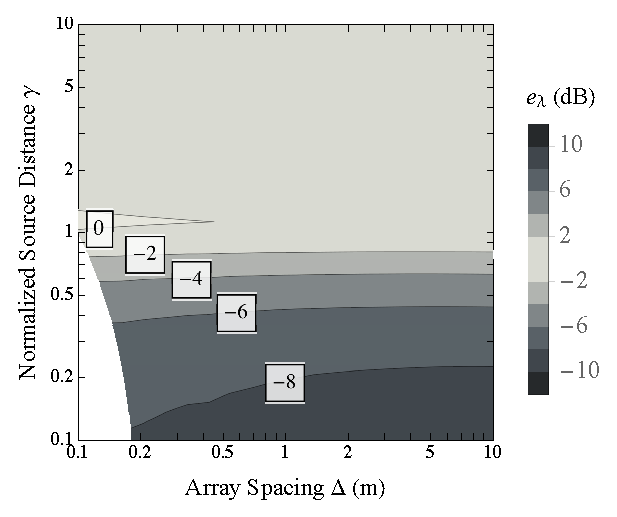
\includegraphics[width=\textwidth]{08_proposed_method/figures/audibleEnergy_contour_xf.eps}
        		\caption{Weighted average method}
        		\label{fig:08_Proposed_Method:Level_Errors:XF}
    	\end{subfigure}
	\hfill
	\begin{subfigure}[b]{0.49\textwidth}
        		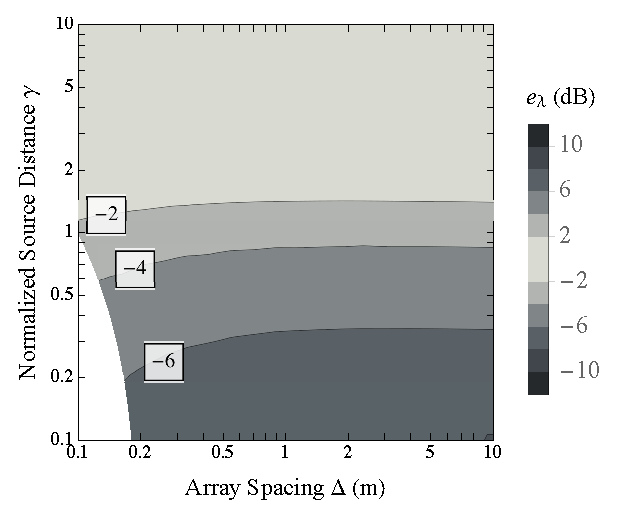
\includegraphics[width=\textwidth]{08_proposed_method/figures/audibleEnergy_contour_validhybrid.eps}
        		\caption{Proposed method}
        		\label{fig:08_Proposed_Method:Level_Errors:Hybrid}
    	\end{subfigure}
	
    	\caption[Contour plots of level errors for each interpolation method.]{
	Level errors $e_\lambda$ for microphone spacing $\Delta$ and normalized source distance $\gamma$.
  Contour lines are drawn every $2$~dB.}
    	\label{fig:08_Proposed_Method:Level_Errors}
\end{figure*}

For the proposed method, a similar problem is encountered.
Note that, for interior sources, typically only one microphone will be valid for any given listening position, and, in such cases, the signals from that microphone are used ``as is'' for the upper portion of the frequency range (see \eqnref{eq:08_Proposed_Method:HybridFilters}).
However, as discussed above, for those listening positions, the amplitude of the signals should increase, since the source will be closer to the listener than it is to the microphone. %%NOTE%% prove this?
So again, it is unsurprising that the proposed method does not achieve a sufficient reproduced level for interior sources.

These errors may be particularly detrimental to a listener's perception of source distance as the listener navigates closer to a source since one of the primary distance cues humans expect is an increase in level \citep[section 3.1.1]{Zahorik2005}.
Consequently, the impact of these errors on a listener's perception of distance should be investigated, although it is outside the scope of this work to do so.

From \figref{fig:08_Proposed_Method:Level_Errors:Hybrid}, we note that the proposed method achieves a minor improvement ($\sim2$~dB) over the weighted average method for far interior sources, approximately $\gamma < 0.4$.
This is primarily due to the exclusion of the invalid microphone by the proposed method, which prevents the comb-filtering introduced by the weighted average method which decreases the average level.
However, the proposed method yields a minor degradation compared to the weighted average method for $\gamma \approx 1$.

As the behavior seen in these plots appears consistent and predictable, one might expect that it would be straightforward to correct with a gain factor, especially for the proposed method since an estimate of the source position is already required for the microphone validity calculation.
However, such a correction would not be viable for sound fields consisting of more than a single source, since, the levels of exterior sources are currently reproduced accurately, and any gain correction would corrupt those sources' signals.

% Coloration

Spectral errors (as defined in \secref{sec:04_Auditory_Models:Coloration_Metrics:ABSE}) for each method are shown in \figref{fig:08_Proposed_Method:Spectral_Errors}.
From these plots, we see that, at large spacings ($\Delta > 0.5$~m) with an interior source ($\gamma < 1$), the proposed method achieves significantly ($\sim 4$~dB) smaller spectral errors than the weighted average method.
This too is primarily due to the exclusion of the invalid microphone from the navigation calculation, which prevents any comb-filtering in the proposed method.

\begin{figure*}[t]
    	\centering
    	\begin{subfigure}[b]{0.49\textwidth}
        		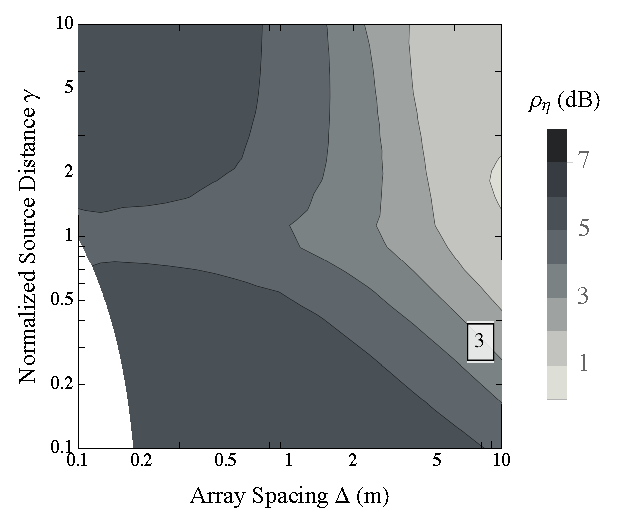
\includegraphics[width=\textwidth]{08_proposed_method/figures/scharer2009_contour_xf.eps}
        		\caption{Weighted average method}
        		\label{fig:08_Proposed_Method:Spectral_Errors:XF}
    	\end{subfigure}
	\hfill
	\begin{subfigure}[b]{0.49\textwidth}
        		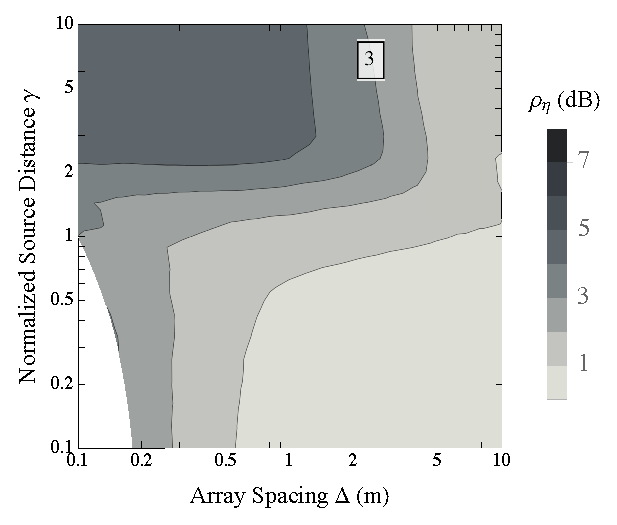
\includegraphics[width=\textwidth]{08_proposed_method/figures/scharer2009_contour_validhybrid.eps}
        		\caption{Proposed method}
        		\label{fig:08_Proposed_Method:Spectral_Errors:Hybrid}
    	\end{subfigure}
	
    	\caption[Contour plots of spectral errors for each interpolation method.]{
	Spectral errors $\rho_\eta$ for microphone spacing $\Delta$ and normalized source distance $\gamma$.
  Contour lines are drawn every $1$~dB.}
    	\label{fig:08_Proposed_Method:Spectral_Errors}
\end{figure*}

Additionally, at small microphone spacings ($\Delta < 0.5$~m) with an exterior source ($\gamma > 1$), the proposed method achieves slightly ($\sim 1$~dB) smaller spectral errors than the weighted average method.
This is due to the widening (as $\Delta$ decreases) of the frequency range over which the regularized least-squares interpolation filters achieve a nearly flat frequency response (see \figref{fig:08_Proposed_Method:Azimuth_Dependence}). % (cf.~\citet[Fig.~4b]{TylkaChoueiri2016}).
As specified in \eqnref{eq:08_Proposed_Method:Hybrid_XO_Freq}, for $P = 2$ microphones, the crossover frequency increases with decreasing $\Delta$, since $r_1 r_2 \propto \Delta^2$.
At large microphone spacings ($\Delta > 0.5$~m) with an exterior source ($\gamma > 1$), the proposed and weighted average methods perform comparably.

% Localization

Localization errors (as computed with \eqnref{eq:04_Auditory_Models:Localization_Error} for the localization model described in \secref{sec:05_Proposed_Models:Localization_Model}) for each method are shown in \figref{fig:08_Proposed_Method:Localization_Errors}.
From these plots, we see that, at large spacings ($\Delta > 0.5$~m) with an interior source ($\gamma < 1$), the proposed method achieves significantly (i.e., at least $10^\circ$) smaller localization errors than the weighted average method.
This too is primarily due to the exclusion of the invalid microphone from the navigation calculation, which prevents any corruption of the localization information by the invalid microphone.

\begin{figure*}[t]
    	\centering
    	\begin{subfigure}[b]{0.49\textwidth}
        		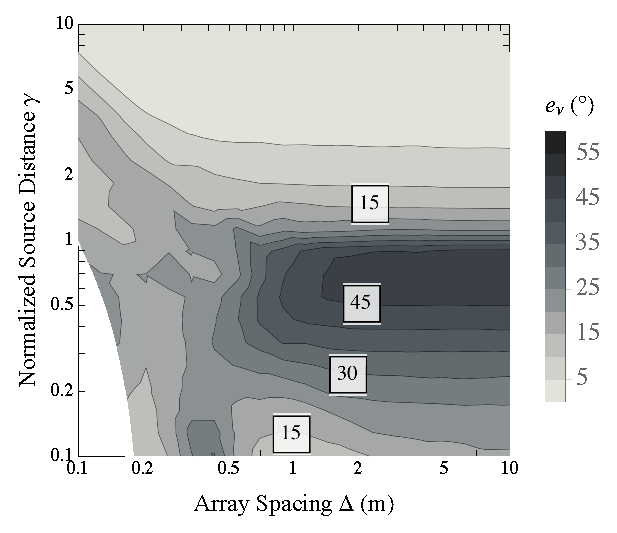
\includegraphics[width=\textwidth]{08_proposed_method/figures/tylka2017_contour_xf.eps}
        		\caption{Weighted average method}
        		\label{fig:08_Proposed_Method:Localization_Errors:XF}
    	\end{subfigure}
	\hfill
	\begin{subfigure}[b]{0.49\textwidth}
        		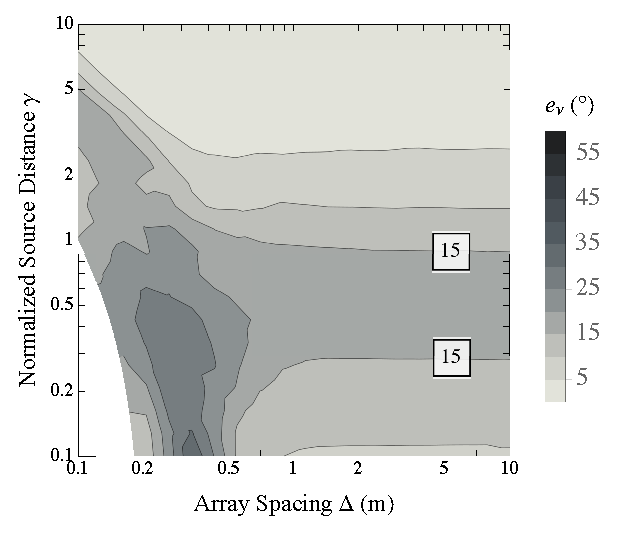
\includegraphics[width=\textwidth]{08_proposed_method/figures/tylka2017_contour_validhybrid.eps}
        		\caption{Proposed method}
        		\label{fig:08_Proposed_Method:Localization_Errors:Hybrid}
    	\end{subfigure}
	
    	\caption[Contour plots of localization errors for each interpolation method.]{
	Predicted localization errors $e_\nu$ for microphone spacing $\Delta$ and normalized source distance $\gamma$.
  Contour lines are drawn every $5^\circ$.}
    	\label{fig:08_Proposed_Method:Localization_Errors}
\end{figure*}

From \figref{fig:08_Proposed_Method:Localization_Errors:Hybrid}, we see that, compared to the weighted average method (see \figref{fig:08_Proposed_Method:Localization_Errors:XF}), the proposed method incurs larger localization errors ($e_\nu > 20^\circ$) for $\Delta < 0.5$~m and $\gamma < 1$ (bottom left corner of the plot).
This penalty may not be too limiting, however, as these values of $\Delta$ and $\gamma$ correspond to sources very near to the origin ($s_0 < 0.25$~m), and in any case, microphone spacings less than $0.5$~m may be impractical.

% Diffuseness

In \figref{fig:08_Proposed_Method:Diffuseness_Errors}, we plot diffuseness errors (as defined in \secref{sec:04_Auditory_Models:Diffuseness_Parameter}) for each method.
For the weighted average method, we see that the diffuseness of the reproduced signals for interior sources ($\gamma < 1$) is too large.
This is due to the increasingly conflicting localization information in the combined signal as $\gamma$ decreases, as illustrated in \figref{fig:08_Proposed_Method:Effective_Sources}.
Consequently, for such interior sources, not only is the localization accuracy degraded, but also the reproduced signals become more diffuse.
For the proposed method, however, the diffuseness is reproduced accurately (i.e., $|e_\Psi| < 0.1$) over almost all conditions, with the exception of at very small $\gamma$ and $\Delta$ (bottom left corner of \figref{fig:08_Proposed_Method:Diffuseness_Errors:Hybrid}).

\begin{figure*}[t]
    	\centering
    	\begin{subfigure}[b]{0.49\textwidth}
        		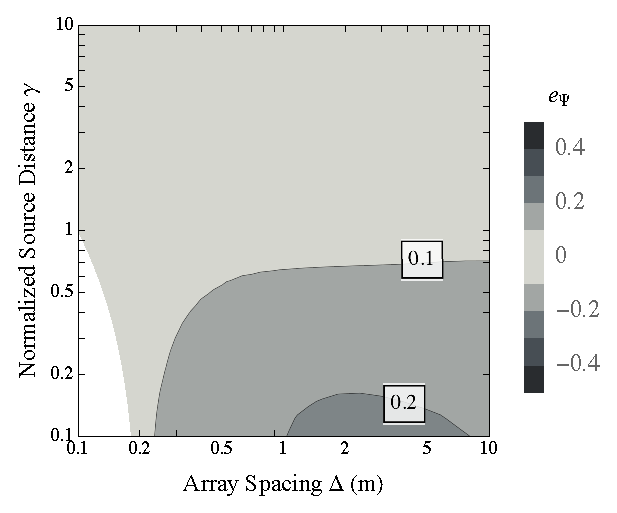
\includegraphics[width=\textwidth]{08_proposed_method/figures/merimaa2005_d_contour_xf.eps}
        		\caption{Weighted average method}
        		\label{fig:08_Proposed_Method:Diffuseness_Errors:XF}
    	\end{subfigure}
	\hfill
	\begin{subfigure}[b]{0.49\textwidth}
        		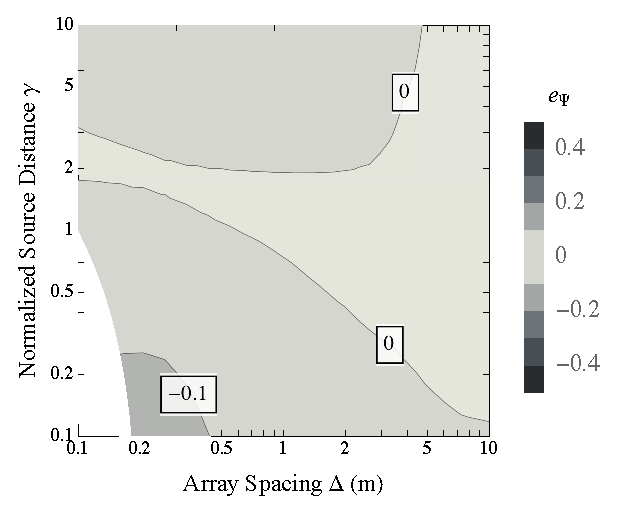
\includegraphics[width=\textwidth]{08_proposed_method/figures/merimaa2005_d_contour_validhybrid.eps}
        		\caption{Proposed method}
        		\label{fig:08_Proposed_Method:Diffuseness_Errors:Hybrid}
    	\end{subfigure}
	
    	\caption[Contour plots of diffuseness errors for each interpolation method.]{
	Diffuseness errors $e_\Psi$ for microphone spacing $\Delta$ and normalized source distance $\gamma$.
  Contour lines are drawn in increments of $0.1$.}
    	\label{fig:08_Proposed_Method:Diffuseness_Errors}
\end{figure*}

%% Order Dependence %%
\subsection{Order dependence}\label{sec:08_Proposed_Method:Order_Dependence}
To further explore the performance of these methods, we plot, in \figref{fig:08_Proposed_Method:Order_Errors}, errors in each metric for a source distance of $s_0 = 1$~m and for input ambisonics orders $L_\textrm{in} = 1,2,\dots,6$.
Since $L_\textrm{out} = 1$ in all cases, the weighted average method is only plotted for $L_\textrm{in} = L_\textrm{out} = 1$.

\begin{figure*}[t]
    	\centering
	\begin{subfigure}[b]{0.49\textwidth}
        		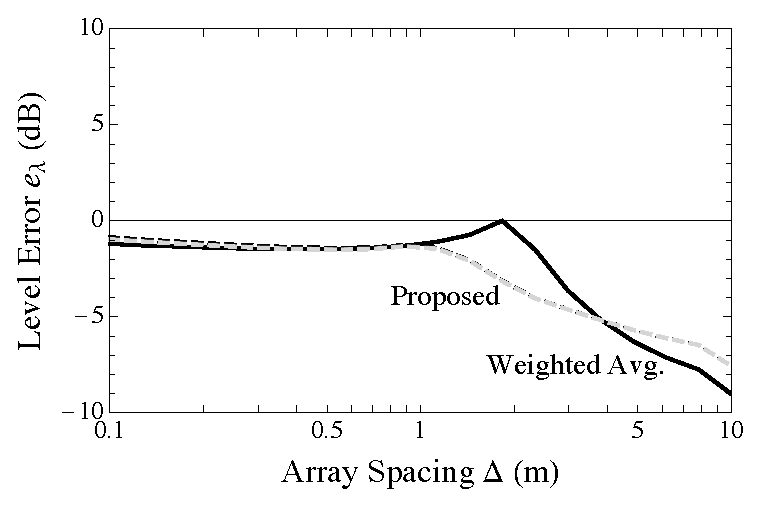
\includegraphics[width=\textwidth]{08_proposed_method/figures/audibleEnergy_order.eps}
        		\caption{Level errors $e_\lambda$}
        		\label{fig:08_Proposed_Method:Level_Errors:Order}
    	\end{subfigure}
	\hfill
    	\begin{subfigure}[b]{0.49\textwidth}
        		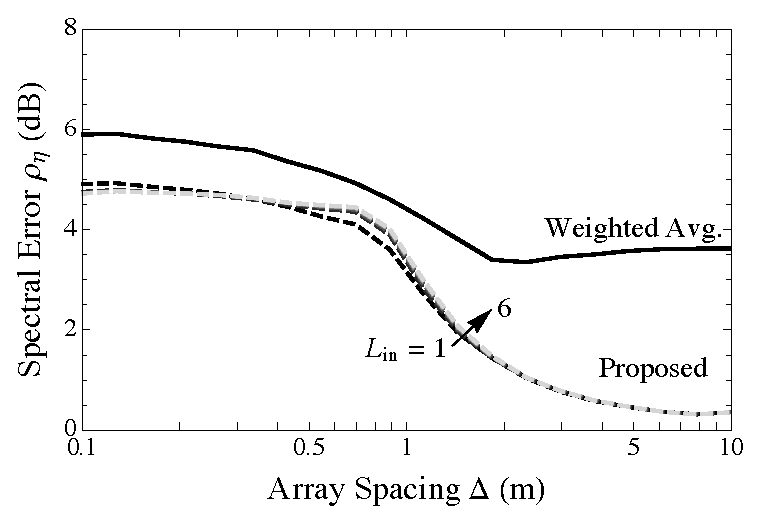
\includegraphics[width=\textwidth]{08_proposed_method/figures/scharer2009_order.eps}
        		\caption{Spectral errors $\rho_\eta$}
        		\label{fig:08_Proposed_Method:Spectral_Errors:Order}
    	\end{subfigure}
	
	\vspace{0.5cm}
	\begin{subfigure}[b]{0.49\textwidth}
        		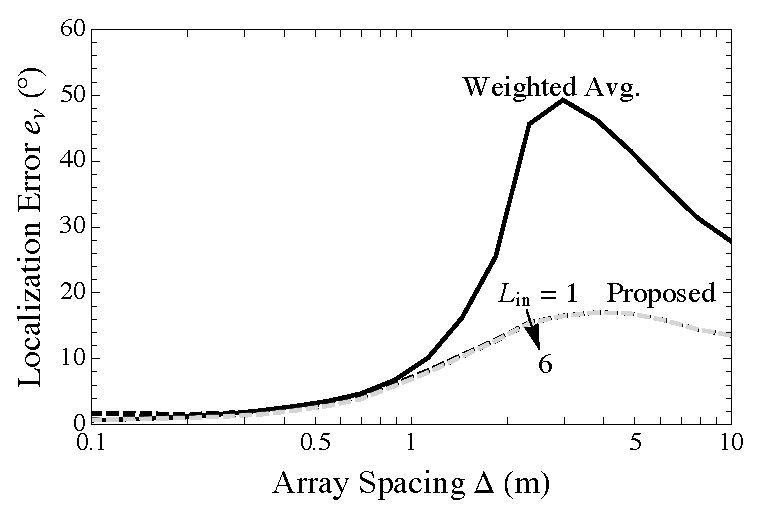
\includegraphics[width=\textwidth]{08_proposed_method/figures/tylka2017_order.eps}
        		\caption{Localization errors $e_\nu$}
		\label{fig:08_Proposed_Method:Localization_Errors:Order}
    	\end{subfigure}
	\hfill
    	\begin{subfigure}[b]{0.49\textwidth}
        		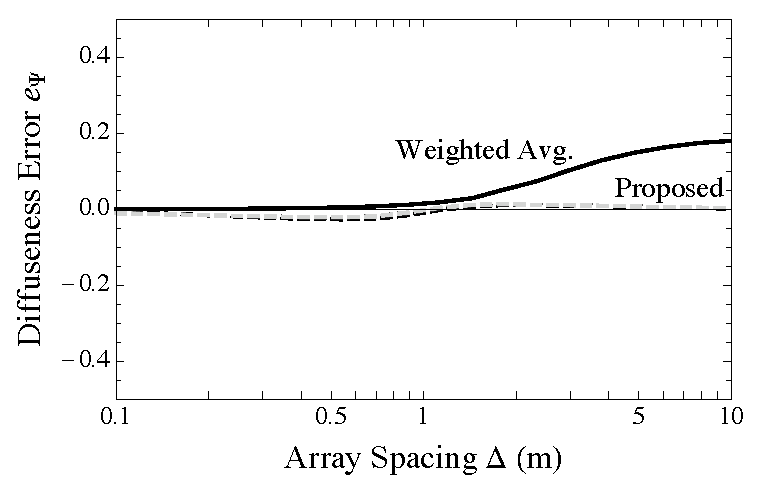
\includegraphics[width=\textwidth]{08_proposed_method/figures/merimaa2005_d_order.eps}
        		\caption{Diffuseness errors $e_\Psi$}
		\label{fig:08_Proposed_Method:Diffuseness_Errors:Order}
    	\end{subfigure}
	
    	\caption[Order dependence plots for each interpolation method.]{
	Errors for various microphone spacings $\Delta$ with a fixed source distance $s_0 = 1$~m.
	Errors are plotted for the weighted average method (solid curves) and the proposed method (dashed curves).
	For the proposed method only, six input ambisonics orders are shown: $L_\textrm{in} = 1$ (black) to $L_\textrm{in} = 6$ (lightest gray).}
    	\label{fig:08_Proposed_Method:Order_Errors}
\end{figure*}

From these figures, we immediately see that virtually all errors incurred by the proposed method are identical at all orders.
This result is somewhat surprising, as one might expect higher-order recordings to produce a more accurate interpolated sound field.
Evidently, however, the input ambisonics order does not significantly affect the performance of the proposed method.
This insensitivity to input order is largely due to the order-independent choice of critical frequency, $k_0$, as given in \eqnref{eq:08_Proposed_Method:Hybrid_XO_Freq}.
Potentially, this critical frequency could be optimized to yield improved accuracy as input order increases, at least over a range of array spacings or source positions.
This is a topic for further development.

In \figref{fig:08_Proposed_Method:Spectral_Errors:Order}, we see that, for microphone spacings $0.4 \leq \Delta \leq 1.5$~m, increasing the input order yields increased spectral coloration.
This behavior can be attributed to the mismatch between the near-field compensation filters (given in \eqnref{eq:02_Acoustical_Theory:NearField_HPF}) and the actual low-frequency amplification caused by the near-field effect, as the magnitude of this mismatch increases with order (cf.~\citet[Fig.~6]{Daniel2003b}).
However, at smaller microphone spacings ($\Delta < 0.3$~m), the opposite effect is observed: increasing the order yields a slight improvement in spectral errors.
This is due to the higher-order terms yielding a more accurate estimate of the sound field at the listening position, although this effect is evidently very minor.

In terms of the other three metrics, we see that, for $\Delta < 1$~m, the performance of the proposed method is already nearly optimal (in terms of level, localization, and diffuseness only) with $L_\textrm{in} = 1$.
This implies that the regularized least-squares interpolation filters do not improve the performance of the proposed method by any of these metrics beyond that achieved by the weighted average method; evidently, the dominant effect of these filters is to decrease spectral errors.
For $\Delta > 1$~m, on the other hand, the performance of the proposed method is improved significantly compared to the weighted average method.
This demonstrates that any improvement seen by the proposed method in terms of these metrics (level, localization, or diffuseness) must be primarily due to the exclusion of invalid microphones from the interpolation calculation.

Overall, the results shown in \figref{fig:08_Proposed_Method:Order_Errors} reaffirm our previous finding that the proposed method tends to outperform the weighted average method for interior sources ($\Delta/2 > s_0 = 1$~m).
In \figref{fig:08_Proposed_Method:Level_Errors:Order}, we see that only in a particular range of microphone spacings does the weighted average method outperform the proposed method; beyond approximately $\Delta = 4$~m, the proposed method outperforms the weighted average method.
By all other metrics (\figrefthru{fig:08_Proposed_Method:Spectral_Errors:Order}{fig:08_Proposed_Method:Diffuseness_Errors:Order}), however, the proposed method outperforms the weighted average method at all spacings $\Delta \geq 1$~m.